\documentclass[a4paper, 12pt]{article}
\usepackage[utf8]{inputenc}
\usepackage{amsmath,amsfonts,amsthm,amssymb,longtable,listings,graphicx, float, epstopdf, textcomp}
\usepackage{mathtools}
\usepackage[finnish]{babel}
\usepackage{tikz}
\usepackage{cite}
\usetikzlibrary{positioning}
\renewcommand{\contentsname}{Sisällysluettelo}
\renewcommand{\abstractname}{Abstrakti}
\theoremstyle{definition}
\newtheorem{mydef}{Määritelmä}
\newtheorem{huom}{Huomautus}
\newtheorem{lemma}{Lemma}
\newtheorem{example}[mydef]{Esimerkki}
\theoremstyle{plain}
\newtheorem{teor}[mydef]{Lause}


\lstset{basicstyle=\small, frame=single}

\begin{document}

\title{Graafien automorfismiryhmät}
\author{Juuso Valli}
\date{25. 4. 2018}

\maketitle

\begin{abstract}
Määritellään graafien automorfismiryhmät, selvitetään joidenkin graafiluokkien automorfismiryhmät, todistetaan Fruchtin teoreema uudella konstruktiolla.
\end{abstract}

\tableofcontents

\newpage

\section{Määritelmiä ja merkintöjä}

Olkoon $V$ äärellinen joukko. Olkoon $E(V) = \{\{u, v\}\;|\;u, v \in V, u \neq v\}$ joukon $V$ alijoukkojen joukko, jonka jäsenet sisältävät täsmälleen kaksi eri solmua.
Olkoon \emph{graafi} $G = (V, E), E \subseteq E(V)$. Joukkoa $V$ kutsutaan graafin $G$ \emph{solmuiksi}, ja joukkoa $E$ kutsutaan \emph{kaariksi}. Solmuja joiden välillä on kaari kutsutaan \emph{naapureiksi}. Annetun solmun kaikkien naapureiden joukkoa kutsutaan solmun \emph{naapurustoksi}. Solmut eivät sisälly omaan naapurustoonsa. Annetun graafin solmujoukosta kätetään merkintää $V_G$, ja kaarijoukosta merkintää $E_G$.
Kaaresta $\{u, v\}$ käytetään merkintää $uv$. Huomaa, että näillä merkinnöillä $uv = vu$.
Yksinkertaisuuden vuoksi solmuista käytetään myös merkintää $v \in G$ merkinnän $v \in V_G$ sijaan.

Olkoot $G$ ja $H$ graafeja. Graafit $G$ ja $H$ ovat \emph{isomorfiset} $G \simeq H$ mikäli on olemassa bijektio $f: V_G \rightarrow V_H$ siten, että
\begin{center}
\begin{math}
uv \in E_G \Longleftrightarrow f(u)f(v) \in E_H
\end{math}
\end{center}
kaikilla $u, v \in G$.

Tällaisia bijektioita kutsutaan \emph{isomorfismeiksi}.

Graafin $G$ \emph{automorfismit} ovat sen isomorfismeja itsensä kanssa. Triviaalisti nähdään, että identiteettikuvaus on kaikkien graafien automorfismi, mutta graafeilla voi olla myös muita automorfismeja.

\begin{example}
\label{ex:d4}
Olkoon graafi $G = (\{v_1, v_2, v_3, v_4\}, \{v_1v_2, v_2v_3, v_3v_4, v_4v_1\})$.

\begin{center}
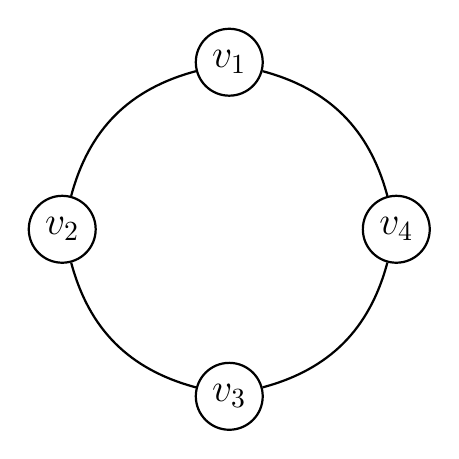
\begin{tikzpicture} [auto, node distance=3cm, every loop/.style={},
                    thick,solmu/.style={circle,draw,font=\sffamily\Large\bfseries}]

\node[solmu] (1) {$v_1$};
\node[solmu] (2) [below left of=1] {$v_2$};
\node[solmu] (3) [below right of=2] {$v_3$};
\node[solmu] (4) [below right of=1] {$v_4$};

 \path[every node/.style={font=\sffamily\small}]
    (1) edge [bend right] node[left] {} (2)
    (2) edge [bend right] node[left] {} (3)
    (3) edge [bend right] node[right] {} (4)
    (4) edge [bend right] node[right] {} (1);
\end{tikzpicture}
\end{center}

Olkoon kuvaus $f: V_G \rightarrow V_G, f(v_1) = v_2, f(v_2) = v_3, f(v_3) = v_4, f(v_4) = v_1$. Kuvaus $f$ on selvästi bijektio. Se, että kuvaus $f$ on automorfismi voidaan tarkistaa suoraan määritelmästä.

\begin{center}
\begin{tabular} {l l l}
$E_G$ & $f(u)f(v)$ & $f^{-1}(u)f^{-1}(v)$ \\
\hline
$v_1v_2$ & $ v_2v_3$ & $v_4v_1$ \\
$v_2v_3$ & $ v_3v_4$ & $v_1v_2$ \\
$v_3v_4$ & $v_4v_1$ & $v_2v_3$ \\
$v_4v_1$ & $v_1v_2$ &  $v_3v_4$ \\
\end{tabular}

\end{center}
\end{example}

\begin{huom}
Kirjallisuudessa käytetään merkintää $G$ sekä ryhmistä että graafeista. Väärinkäsitysten välttämiseksi sovitaan, että $G$ viittaa aina graafiin ja ryhmästä käytetään merkintää $R$.
\end{huom}

Olkoon $R$ ryhmä, jolla on aliryhmät $H$ ja $K$. 

Ryhmä $R$ on aliryhmiensä \emph{suora tulo} (merkitään $R = H \times K$) mikäli seuraavat kolme ehtoa ovat voimassa:
\begin{center}
\begin{math}
R = HK, H \cap K = \{ 1\}, hk = kh \; \forall h \in H, k \in K
\end{math}
\end{center}

Ryhmä $R$ on aliryhmiensä \emph{(sisäinen) puolisuora tulo} (merkitään $R = H \rtimes K$) mikäli seuraavat kolme ehtoa ovat voimassa:
\begin{center}
\begin{math}
R = HK,  H \cap K = \{ 1\}, H \trianglelefteq R
\end{math}
\end{center}

Olkoot $H, K$ mielivaltaisia ryhmiä, ja ryhmähomomorfismi $\tau: K \rightarrow \mathrm{Aut}(H)$. Merkitään $\tau_k = f(k)$. Ryhmien \emph{(ulkoinen) puolisuora tulo}, merkitään $H \rtimes_\tau K$, on karteesinen tulo $H \times K$ varustettuna tulolla $(h_1, k_1)(h_2, k_2) = (h_1\tau_{k_1}(h_2), k_1k_2)$.

Määritelmät ovat mukailtuja lähteistä \cite{ryhmateoria}\cite{grapththeory}.

\section{Automorfismiryhmä}

Olkoon $\mathrm{Aut}(G)$ graafin $G$ automorfismien joukko.

\begin{lemma}
\label{lemma:binaarirelaatio}
Kuvausten kompositio on binäärioperaatio $\circ : \mathrm{Aut}(G) \times \mathrm{Aut}(G) \rightarrow \mathrm{Aut}(G)$.
\begin{proof}
Olkoot $u, v \in G$. Olkoon $f, g \in \mathrm{Aut}(G)$.
\begin{center}
\begin{math}
uv \in E_G \xLeftrightarrow{g \in \mathrm{Aut}(G)} g(u)g(v) \in E_G  \xLeftrightarrow{f \in \mathrm{Aut}(G)} f(g(u))f(g(v)) \in E_G 
\end{math}
\end{center}
joten $f \circ g \in \mathrm{Aut}(G)$.
\end{proof}
\end{lemma}

\begin{lemma}
\label{lemma:identiteetti}
Jokaisella graafilla on identiteettikuvaus, joka on automorfismi.
\begin{proof}
Olkoot $u, v \in G$. Olkoon $\mathrm{id}: V_G \rightarrow V_G, \mathrm{id}(x) = x \; \forall x \in V_G$.
\begin{center}
\begin{math}
uv \in E_G \xLeftrightarrow{\mathrm{id}(x) = x} \mathrm{id}(u)\mathrm{id}(v) \in E_G  
\end{math}
\end{center}
joten $\mathrm{id} \in \mathrm{Aut}(G)$.
\end{proof}
\end{lemma}

\begin{lemma}
\label{lemma:kaanteiskuvaus}
Automorfismin $f$ käänteiskuvaus $f^{-1}$ on automorfismi.
\begin{proof}
Olkoot $u, v \in G$.
\begin{center}
\begin{math}
f^{-1}(u)f^{-1}(v) \in E_G \xLeftrightarrow{f \in \mathrm{Aut}(G)} f(f^{-1}(u))f(f^{-1}(v)) \in E_G \Leftrightarrow uv \in E_G
\end{math}
\end{center}
joten $f^{-1} \in \mathrm{Aut}(G)$.
\end{proof}
\end{lemma}

\begin{teor}
Pari $(\mathrm{Aut}(G), \circ)$ on ryhmä.
\begin{proof}
Lemman \ref{lemma:binaarirelaatio} mukaan $\circ$ on $\mathrm{Aut}(G)$:n binäärioperaatio. Assosiatiivisuus on selvä kuvausten komposition assosiatiivisuuden perusteella. Lemman \ref{lemma:identiteetti} mukaan jokainen $\mathrm{Aut}(G)$ sisältää identiteettikuvauksen $\mathrm{id}$, joka on ryhmän neutraalialkio. Lemman \ref{lemma:kaanteiskuvaus} mukaan jokaisella automorfismilla $f$ on käänteisalkio $f^{-1} \in \mathrm{Aut}(G)$ siten, että $f \circ f^{-1} = \mathrm{id}$.
\begin{center}
\begin{math}
\end{math}
\end{center}
\end{proof}
\end{teor}

Graafin automorfismiryhmää kutsutaan myös graafin symmetriaryhmäksi.

\begin{huom}
Graafien automorfismiryhmät eivät yleisesti ole kommutatiivisia.\\
Tämä nähdään helposti vastaesimerkin kautta. Tarkastellaan esimerkin \ref{ex:d4} mukaista graafia. Olkoon $f$ esimerkissä esitetty automorfismi. Olkoon kuvaus $g: V_G \rightarrow V_G, g(v_1) = v_1, g(v_2) = v_4, g(v_3) = v_3, g(v_4) = v_2$. Kuvaus $g$ on selvästi myös graafin $G$ automorfismi. Mikäli automorfismiryhmä olisi kommutatiiviinen, olisi $f \circ g = g \circ f$. Kirjoittamalla kuvaukset auki nähdään, että $f \circ g(v_1) = f(g(v_1)) = f(v_1) = v_2$, mutta toisaalta $g \circ f (v_1) = g(f(v_1)) = g(v_2) = v_4$, mistä seuraa ristiriita.
\end{huom}

\begin{example}
Esimerkin \ref{ex:d4} mukaisen graafin symmetriaryhmä $\mathrm{Aut}(G)$ on isomorfinen diedriryhmän $D_4$ kanssa. Yleisemmin $n$:n solmun rengasgraafi on isomorfinen diedriryhmän $D_n$ kanssa.

Olkoon $G$ $n$:n solmun rengasgraafi, ja $v_i$ sen $i$:nnes solmu jossakin järjes\-tyk\-sessä. Solmujen orientaatiolla tarkoitetaan sitä, ovatko alkiot indeksoitu myötä- vai vastapäivään.

Jokainen automorfismi joko säilyttää solmujen orientaation tai kääntää sen. Tästä voidaan määritellä homomorfismi $\phi: \mathrm{Aut}(G) \rightarrow C_2$, missä $\phi(f) = 0$ mikäli $f$ säilyttää solmujen orientaation, muulloin $\phi(f) = 1$. Homomorfismin $\phi$ ydin $\mathrm{Ker}(\phi) = \{f_i \in \mathrm{Aut}(G), o \leq i < n\;|\;\forall 0 \leq j < n: f_i(v_j) = v_{i + j\; \pmod{ n}}\}$ muodostuu kuvauksista, jotka siirtävät graafin solmuja kään\-tämät\-tä niiden orientaatiota. Tämä on isomorfinen ryhmän $C_n$ kanssa. Olkoot kuvaus $\mathrm{rev} \in \mathrm{Aut}(G):  \mathrm{rev}(v_i) = v_{n - 1 - i}$. Selvästi $\mathrm{rev} \circ \mathrm{rev} = \mathrm{id}$, joten $\langle \mathrm{rev} \rangle$ määrittää kahden alkion aliryhmän, joka leikkaus aliryhmän $\mathrm{Ker}(\phi)$ kanssa on $\mathrm{Ker}(\phi) \cap \langle rev \rangle = \{ \mathrm{id} \}$.

Olkoon $f \in \mathrm{Aut}(G)$ mielivaltainen, ja $0 \leq i < n$ siten, että $f(v_0) = v_i$. Nyt $(f_i^{-1} \circ f)(0) = 0$, eli $(f_i^{-1} \circ f \in \langle \mathrm{rev} \rangle$. Tästä seuraa, että $f$ voidaan esittää muodossa $f = f_i \circ \mathrm{rev}^k$ missä $k \in \{0, 1\}$. Tästä seuraa se, että $\mathrm{Aut}(G) = \mathrm{Ker}(\phi) \langle \mathrm{rev} \rangle$, mistä seuraa edellisten kohtien perusteella se, että $\mathrm{Aut}(G) = \mathrm{Ker}(\phi) \rtimes \langle \mathrm{rev} \rangle \simeq C_n \rtimes_\tau C_2$, jossa $\tau: C_2 \rightarrow \mathrm{Aut}(C_n), \tau(0) = \mathrm{id}, \tau(1) = c_i \mapsto c_{n - 1 - i}$.
\end{example}

\begin{example}
Suoran graafin symmetriaryhmä on $C_2$.

\begin{center}
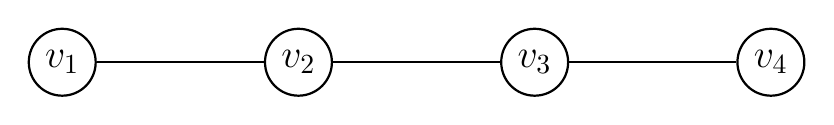
\begin{tikzpicture} [auto, node distance=3cm, every loop/.style={},
                    thick,solmu/.style={circle,draw,font=\sffamily\Large\bfseries}]

\node[solmu] (1) {$v_1$};
\node[solmu] (2) [right of=1] {$v_2$};
\node[solmu] (3) [right of=2] {$v_3$};
\node[solmu] (4) [right of=3] {$v_4$};

 \path[every node/.style={font=\sffamily\small}]
    (1) edge node[left] {} (2)
    (2) edge node[left] {} (3)
    (3) edge node[left] {} (4);
\end{tikzpicture}
\end{center}

Suoran graafin päädyissä olevilla solmujen aste on $1$, ja kaikkien muiden solmujen aste on $2$. Tästä seuraa se, että graafin päätysolmut voidaan kuvata vain päätysolmuihin, sillä isomorfismit säilyttävät solmujen asteen. Yhden päätysolmujen kuvan määrääminen riittää määräämään koko graafin kuvan, joten mahdollisia kuvauksia on vain kaksi: $\mathrm{id}$ ja kuvaus $f$, joka kuvaa solmun $v_i$ solmuksi $v_{n - i + 1}$. Koska $f \circ f = \mathrm{id}$, graafin automorfismiryhmä on $C_2$.
\end{example}

\begin{example}
Täyden graafin $K_n$ symmetriaryhmä on $S_n$.

\begin{center}
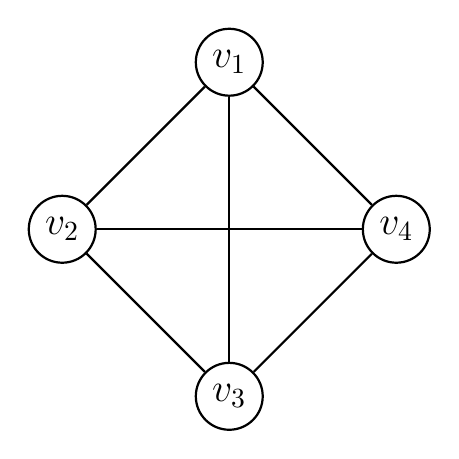
\begin{tikzpicture} [auto, node distance=3cm, every loop/.style={},
                    thick,solmu/.style={circle,draw,font=\sffamily\Large\bfseries}]

\node[solmu] (1) {$v_1$};
\node[solmu] (2) [below left of=1] {$v_2$};
\node[solmu] (3) [below right of=2] {$v_3$};
\node[solmu] (4) [below right of=1] {$v_4$};

 \path[every node/.style={font=\sffamily\small}]
    (1) edge node[left] {} (2)
    (1) edge node[left] {} (3)
    (1) edge node[left] {} (4)
    (2) edge node[left] {} (3)
    (2) edge node[left] {} (4)
    (3) edge node[left] {} (4);
\end{tikzpicture}
\end{center}

Koska jokainen solmu on kaikkien muiden solmujen naapuri, jokainen $K_n$:n bijektio itsensä kanssa on automorfismi. Tästä seuraa se, että graafin $K_n$ automorfismiryhmä on $Sym(K_n) \simeq S_n$.
\end{example}

\begin{example}
\label{example:k_nm}
Täysin kaksijakoisen graafin $K_{nm}, n \neq m$ symmetriaryhmä on $S_n \times S_m$.

\begin{center}
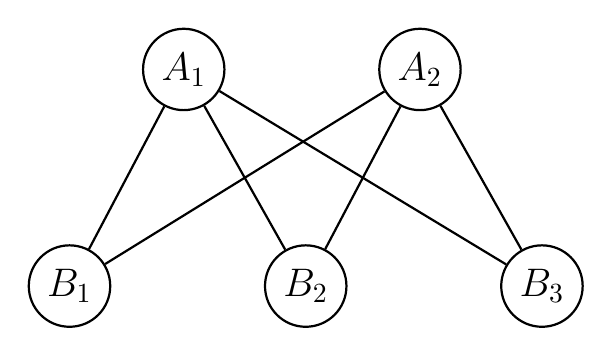
\begin{tikzpicture} [auto, node distance=3cm, every loop/.style={},
                    thick,solmu/.style={circle,draw,font=\sffamily\Large\bfseries}]

\node[solmu] (1) {$A_1$};
\node[solmu] (2) [right of=1] {$A_2$};
\node[solmu] (3) [below left=2cm and 0.7cm  of 1] {$B_1$};
\node[solmu] (4) [right of=3] {$B_2$};
\node[solmu] (5) [right of=4] {$B_3$};

 \path[every node/.style={font=\sffamily\small}]
    (1) edge node[left] {} (3)
    (1) edge node[left] {} (4)
    (1) edge node[left] {} (5)
    (2) edge node[left] {} (3)
    (2) edge node[left] {} (4)
    (2) edge node[left] {} (5);
\end{tikzpicture}
\end{center}

Olkoot $A, B \subset G_v$ graafin ylä- ja alakomponentit. Olkoot $H = \{f \in \mathrm{Aut}(G) : f|_A = \mathrm{id}\}, K = \{f \in \mathrm{Aut}(G) : f|_B = \mathrm{id}\}$. Kumpikin osajoukko on selvästi aliryhmä, sillä $(f \circ g)|_X = \mathrm{id}$ jos $f|_X = \mathrm{id}, g|_X = \mathrm{id}$. Lisäksi nähdään, että $H \cap K = \{ \mathrm{id} \}$.

Määritellään funktion jako seuraavasti:

\begin{center}
\begin{math}
f_X(x) =
\left\{
	\begin{array}{ll}
		f(x)  & \mbox{jos } x \in X \\
		x & \mbox{jos } x \notin X
	\end{array}
\right.
\end{math}
\end{center}

Mielivaltainen automorfismi $f$ voidaan jakaa kahteen osaan joukkojen $A$ ja $B$ mukaan, josta saadaan $f = f_A \circ f_B, f_A \in K, f_B \in H$. Tästä seuraa, että $G = HK$.

Olkoot $h \in H, k \in K$. Tapauksessa $x \in A$:
\begin{center}
\begin{math}
(h \circ k)(x) = (h \circ \mathrm{id})(x) = (\mathrm{id} \circ h)(x) = (k \circ h)(x)
\end{math}
\end{center}

Toisaalta tapauksessa $x \in B$:
\begin{center}
\begin{math}
(h \circ k)(x) = (\mathrm{id} \circ k)(x) = (k \circ \mathrm{id})(x) = (k \circ h)(x)
\end{math}
\end{center}

Eli $hk = kh$. Tästä seuraa, että $\mathrm{Aut}(G) \simeq H \times K = S_n \times S_m$.
\end{example}

\begin{example}
Täysin kaksijakoisen graafin $K_{nn}$ symmetriaryhmä on $ S_n^2 \rtimes C_2 $.

\begin{center}
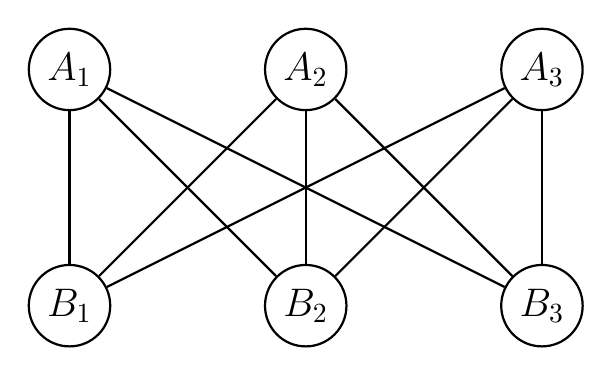
\begin{tikzpicture} [auto, node distance=3cm, every loop/.style={},
                    thick,solmu/.style={circle,draw,font=\sffamily\Large\bfseries}]

\node[solmu] (1) {$A_1$};
\node[solmu] (2) [right of=1] {$A_2$};
\node[solmu] (3) [right of=2] {$A_3$};
\node[solmu] (4) [below of=1] {$B_1$};
\node[solmu] (5) [right of=4] {$B_2$};
\node[solmu] (6) [right of=5] {$B_3$};

 \path[every node/.style={font=\sffamily\small}]
    (1) edge node[left] {} (4)
    (1) edge node[left] {} (5)
    (1) edge node[left] {} (6)
    (2) edge node[left] {} (4)
    (2) edge node[left] {} (5)
    (2) edge node[left] {} (6)
    (3) edge node[left] {} (4)
    (3) edge node[left] {} (5)
    (3) edge node[left] {} (6);
\end{tikzpicture}
\end{center}

Olkoot $A, B \subset G_v$ graafin ylä- ja alakomponenit. Jokaisella automorfismilla joko $f(A) = A$ tai $f(A) = B$. Määritellään kuvaus $\phi: \mathrm{Aut}(G) \rightarrow C_2$, jossa
\begin{center}
\begin{math}
\phi(f) =
\left\{
	\begin{array}{ll}
		0  & \mbox{jos } f(A) = A \\
		1 & \mbox{jos } f(A) = B
	\end{array}
\right.
\end{math}
\end{center}
Kuvaus $\phi$ on selvästi homomorfismi.

Homomorfismin $\phi$ ydin on esimerkin \ref{example:k_nm} nojalla $S_n^2$. Määritellään homomorfismi $\sigma: C_2 \rightarrow \mathrm{Aut}(G)$ siten, että $0$ kuvautuu identiteettikuvauksesi ja $1$ kuvautuu kuvaukseksi, joka vaihtaa $A$:n ja $B$:n alkiot mutta säilyttää niiden sisäisen järjestyksen. Ryhmä $C_2$ operoi sillä joukossa $\mathrm{Aut}(G)$, joten $\mathrm{Aut}(G) \simeq S_n^2 \rtimes_\sigma C_2$.
\end{example}

\begin{example}
Hamming-graafi on graafi, jonka solmut vastaavat $n$:n merkin pituisia binäärijonoja, eli $\mathbb{Z}_2^n$:n alkioita. Kahden solmun välillä on kaari mikäli solmuja vastaavat binäärijonot poikkeavat täsmälleen yhdellä merkillä. Hamming-graafin voidaan ajatella kuvaavan n-ulotteisen hyperkuution kulmia.

\begin{center}
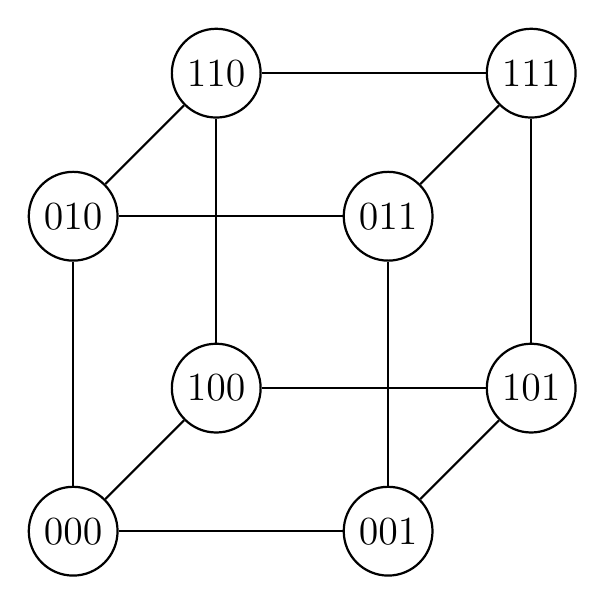
\begin{tikzpicture} [auto, node distance=4cm, every loop/.style={},
                    thick,solmu/.style={circle,draw,font=\sffamily\Large\bfseries}]

\node[solmu] (N000) {$000$};
\node[solmu] (N001) [right of=N000] {$001$};
\node[solmu] (N010) [above of=N000] {$010$};
\node[solmu] (N100) [above right=1cm and 1cm of N000] {$100$};
\node[solmu] (N011) [above of=N001] {$011$};
\node[solmu] (N101) [above right=1cm and 1cm of N001] {$101$};
\node[solmu] (N110) [above right=1cm and 1cm of N010] {$110$};
\node[solmu] (N111) [right of=N110] {$111$};

 \path[every node/.style={font=\sffamily\small}]
    (N000) edge node[left] {} (N001)
    (N000) edge node[left] {} (N010)
    (N000) edge node[left] {} (N100)
    (N001) edge node[left] {} (N011)
    (N001) edge node[left] {} (N101)
    (N010) edge node[left] {} (N110)
    (N010) edge node[left] {} (N011)
    (N100) edge node[left] {} (N101)
    (N100) edge node[left] {} (N110)
    (N110) edge node[left] {} (N111)
    (N101) edge node[left] {} (N111)
    (N011) edge node[left] {} (N111);
\end{tikzpicture}
\end{center}

Tutkitaan hamming-graafien automorfismiryhmää.

Käytetään tässä seuraavia merkintöjä:
\begin{center}
\begin{tabular}{l}
$u + v = (u_1 + v_1, \dots, u_n + v_n) \in \mathbb{Z}_2^n$\\
$1_i \in \mathbb{Z}_2^n$ missä $1_i$:n $i$:s merkki on 1, muut 0.\\
$\bar{0} \in \mathbb{Z}_2^n$ missä kaikki merkit ovat 0.
\end{tabular}
\end{center}
Selvästi $ \forall u \in \mathbb{Z}_2^n: u + u = \bar{0}$.

Olkoot $G$ hamming-graafi ja $f$ sen automorfismi. Olkoot $u \in G$ ja $v = f(u)$. Koska jokainen solmun $u$ naapuri kuvatuu solmun $v$ naapuriksi, yhden merkin muuttaminen alkukuvassa $u$ muuttaa yhden merkin kuvassa $v$. Automorfismi $f$ ei voi muuttaa samaa solmun $v$ merkkiä solmun $u$ naapurustossa, koska muuten $f$ kuvaisi kaksi solmun $u$ naapuria samaksi solmuksi. Voidaan ajatella, että $f$ permutoi merkkien paikkoja solmun $u$ ympäristössä. 

Olkoot $0 < i, j \leq n, i \neq j$. Solmut $u + 1_i$ ja $u+ 1_j$ ovat solmun $u$ naapureita, joiden kuvat poikkeavat solmusta $v$ joillakin indekseillä $i' \neq j'$. Solmun $u$ lisäksi on olemassa vain yksi toinen solmu joka on solmujen $u + 1_i$ ja $u + 1_j$ naapureita: $u + 1_i + 1_j$. Sitä vastaava kuva voidaan esittää kahdella tavalla: $f(u + 1_i + 1_j) = f(u + 1_i) + 1_{j''} = f(u + 1_j) + 1_{i''}$ joillakin indekseillä $i'' \neq j', j'' \neq i'$. Tästä seuraa, että $v + 1_{i'} + 1_{j''} = v + 1_{j'} + 1_{i''} \Leftrightarrow 1_{i'} = 1_{i'} \wedge 1_{j'} = j_{j''}$, eli  automorfismin $f$ muodostamat merkkipermutaatiot eivät riipu solmun $u$ valinnasta. Voidaan siis määritellä kuvaus ${\phi: \mathrm{Aut}(G) \rightarrow S_n}$, joka kuvaa automorfismit niiden merkkipermutaatioiksi.

Olkoot $f_1, f_2 \in \mathrm{Aut}(G)$. 
\begin{center}
\begin{math}
\forall u \in \mathbb{Z}_2^n, 0 < i \leq n: (f_1 \circ f_2)(u + 1_i) = f_1(f_2(u + 1_i))
= f_1(f_2(u) + 1_{\phi(f_2)(i)}) = f_1(f_2(u)) + 1_{(\phi(f_1) \circ \phi(f_2))(i)}
\end{math}
\end{center}
Tästä seuraa, että $\phi(f_1 \circ f_2) = \phi(f_1) \circ \phi(f_2)$, eli kuvaus $\phi$ on homomorfismi.

Tarkastellaan kuvauksen $\phi$ ydintä. Symmetrisen ryhmän $S_n$ neutraalialkio on identiteettikuvaus $\mathrm{id}$. Automorfismin $f$ kuva $\phi(f)$ on identiteettikuvaus jos ja vain jos $ \forall u \in G, 0 < i \leq n: f(u + 1_i) = f(u) + 1_i$. Toisaalta $u = \sum{k \in I} 1_k$ jonkin indeksijoukon $I \subset \{1, \dots , n\}$ yli, joten $f(u) = u + f(\bar{0})$. Solmun $\bar{0}$ mahdolliset kuvat määrävät siis kuvauksen $\phi$ ytimen alkiot. Olkoot $f_1, f_2 \in \mathrm{Ker}(\phi)$. $(f_1 \circ f_2)(u) = u + f_1(\bar{0}) + f_2(\bar{0})$, joten $\mathrm{Ker}(\phi) \simeq C_2^n$. Toisaalta joukko $H = \{f \in \mathrm{Aut}(G) : f(\bar{0}) = \bar{0}\} \simeq S_n$ muodostaa myös $\mathrm{Aut}(G)$:n aliryhmän, sillä pelkät merkkipermutaatiot ovat myös automorfismeja. Koska $H$ ei muuta merkkejä, ja $\mathrm{Ker}(\phi)$ ei permutoi merkkien paikkoja, $H \cap \mathrm{Ker}(\phi) = \{ \mathrm{id} \}$. Koska $\mathrm{Ker}(\phi)$ on homomorfismin ydin, $\mathrm{Ker}(\phi) \trianglelefteq \mathrm{Aut}(G)$.

Automorfismiryhmä $\mathrm{Aut}(G)$ ei sisällä muita aliryhmiä, sillä mielivaltainen automorfismi voidaan esittää edellä mainittujen aliryhmien avulla. Tästä seuraa, että $\mathrm{Aut}(G) = \mathrm{Ker}(\phi) \rtimes H \simeq C_2^n \rtimes_\tau S_n$, jossa $\tau: S_n \rightarrow \mathrm{Aut}(C_2^n)$ siten, että $\phi \circ \tau = \mathrm{id}$.
\end{example}

\begin{example}
Olkoon $G$ seuraava graafi:

\begin{center}
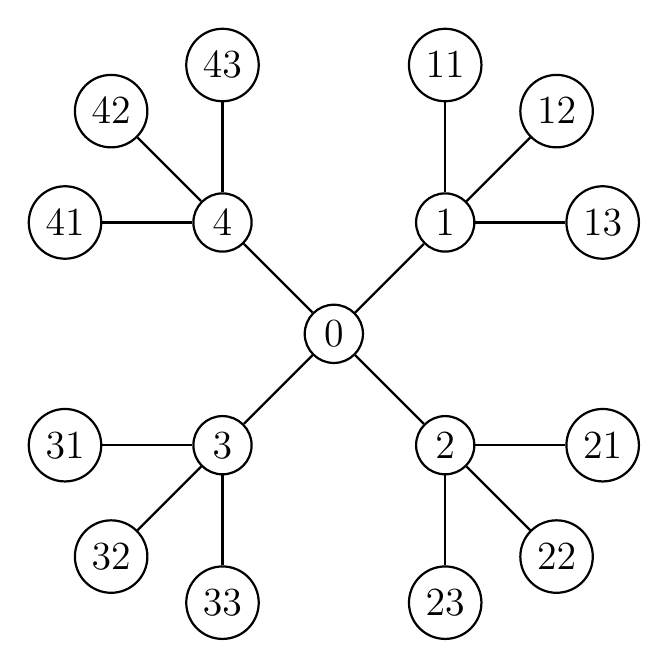
\begin{tikzpicture} [auto, node distance=2cm, every loop/.style={},
                    thick,solmu/.style={circle,draw,font=\sffamily\Large\bfseries}]

\node[solmu] (N0) {$0$};
\node[solmu] (N1) [above right of=N0] {$1$};
\node[solmu] (N2) [below right of =N0] {$2$};
\node[solmu] (N3) [below left of =N0] {$3$};
\node[solmu] (N4) [above left of =N0] {$4$};
\node[solmu] (N11) [above of=N1] {$11$};
\node[solmu] (N12) [above right of =N1] {$12$};
\node[solmu] (N13) [right of =N1] {$13$};
\node[solmu] (N21) [right of=N2] {$21$};
\node[solmu] (N22) [below right of =N2] {$22$};
\node[solmu] (N23) [below of =N2] {$23$};
\node[solmu] (N31) [left of=N3] {$31$};
\node[solmu] (N32) [below left of =N3] {$32$};
\node[solmu] (N33) [below of =N3] {$33$};
\node[solmu] (N41) [left of=N4] {$41$};
\node[solmu] (N42) [above left of =N4] {$42$};
\node[solmu] (N43) [above of =N4] {$43$};

 \path[every node/.style={font=\sffamily\small}]
    (N1) edge node[left] {} (N0)
    (N2) edge node[left] {} (N0)
    (N3) edge node[left] {} (N0)
    (N4) edge node[left] {} (N0)
    (N11) edge node[left] {} (N1)
    (N12) edge node[left] {} (N1)
    (N13) edge node[left] {} (N1)
    (N21) edge node[left] {} (N2)
    (N22) edge node[left] {} (N2)
    (N23) edge node[left] {} (N2)
    (N31) edge node[left] {} (N3)
    (N32) edge node[left] {} (N3)
    (N33) edge node[left] {} (N3)
    (N41) edge node[left] {} (N4)
    (N42) edge node[left] {} (N4)
    (N43) edge node[left] {} (N4);
\end{tikzpicture}
\end{center}

Käytetään alkiosta $0$ termiä runko, alkioista $0 \dots 4$ termiä oksa ja muista alkioista termiä lehti. Helposti nähdään, että graafin $G$ automorfismit säilyttävät rungon paikallaan, kuvaavat oksat oksiksi ja lehdet lehdiksi. Lisäksi saman oksan lehdet pysyvät yhdessä. Oksat voivat kaikki vaihtaa paikkaa keskenään, joten jokainen automorfismi $f$ määrää oksien jonkin permutaation. 
Olkoon kuvaus $\phi: \mathrm{Aut}(G) \rightarrow S_4$ siten, että $f \in \mathrm{Aut}(G)$ kuvautuu oksien permutaatioksi. Kuvaus $\phi$ on selvästi homomorfismi, ja sen ytimessä olevat automorfismit säilyttävät siis oksat paikallan. Koska lehtiä voi permutoida vapaasti annetun oksan ympärillä ja lehtiryppäät eivät vaikuta toisiinsa, koko ydin saadaan lehtien permutaatioryhmien suorana tulona: $\mathrm{Ker}(\phi) \simeq S_3^4$. 

Määritellään homomorfismi $\sigma: S_4 \rightarrow \mathrm{Aut}(G)$ siten, että $S_4$:n alkio kuvautuu automorfismiksi joka permutoi oksia syötealkion tavoin, mutta säilyttää lehtien luonnollisen järjestyksen. Ryhmä $S_4$ operoi tällä homomorfismilla joukossa $\mathrm{Aut}(G)$, joten saadaan $\mathrm{Aut}(G) \simeq S_3^4 \rtimes S_4$.
\end{example}

\newpage

\section{Fruchtin teoreema}

\begin{teor}
\label{frucht}
Olkoon $R$ äärellinen ryhmä. On olemassa äärellinen graafi $G$ siten, että $\mathrm{Aut}(G) \simeq R$.
\begin{proof}
Tutkitaan ensin väritettyä ja suunnattua Cayleyn graafia, ja esitellään menetelmä jolla voidaan siirtyä värittömiin ja suuntaamattomiin graafeihin. Väritetyn ja suunnatun graafin automorfismit määritellään ilmeisellä tavalla.

Olkoot $S$ ryhmän $R$ generaattorijoukko ja $C$ $|S|$:n värin joukko. Määri\-tellään bijektio $\lambda: S \rightarrow C$, joka määrittää siis joukon $R$ generaattoreiden värityksen.

Olkoon $G$ suunnattu ja väritetty graafi, jonka solmut vastaavat ryhmän $R$ alkioita bijektion $\alpha: R \rightarrow V_G$ avulla. Merkitään $v_a = \alpha(a)$. Graafin suunnatut kaaret ovat $E_G = \{ (a, ab) : a \in R, b \in S\}$. Annetun kaaren $(a, ab)$ väri on $\lambda(b)$.

Määritellään ryhmän $R$ mielivaltaisia alkioita $a$ vastaavat kuvaukset $f_a: G \rightarrow G, f_a(v_b) = v_{ab}$. Kuvaus $f_a$ on automorfismi, sillä
\begin{center}
\begin{tabular}{r l}
$uv \in E_G$ & $\Leftrightarrow \exists b \in S: \alpha^{-1}(u) = \alpha^{-1}(v)b$ \\
& $\Leftrightarrow \exists b \in S: a\alpha^{-1}(u) = a\alpha^{-1}(v)b$ \\
& $\Leftrightarrow f_a(u)f_a(v) \in E_G$\\
\end{tabular}
\end{center}

Olkoon $f \in \mathrm{Aut}(G)$ mielivaltainen. Yksittäisen solmun kuva riittää mää\-rää\-mään kuvauksen $f$ täysin, sillä kuvan $f(v_a)$ naapureilla on aina täsmälleen yksi mahdollinen kuva joka säilyttää graafin kaaret. Selvästi $\exists b \in R: f(v_a) = v_{ba}$ joten $f = f_b$.

Edellisen nojalla voimme määritellä kuvauksen $\phi: R \rightarrow \mathrm{Aut}(G): \phi(a) = f_a$, joka on isomorfismi.

Tutkitaan lisäksi miten voidaan konstruoida väritön ja suuntaamaton graafi $G'$ jolla $\mathrm{Aut}(G') \simeq \mathrm{Aut}(G) \simeq R$. 
Korvataan graafin väritetyt ja suunnatut kaaret aligraafeilla, jotka ovat epäsymmetrisiä ja sellaisia, että vain samaa väriä vastaavat aligraafit ovat isomorfisia keskenään. Esimerkiksi seuraavalla tavalla:

\begin{center}
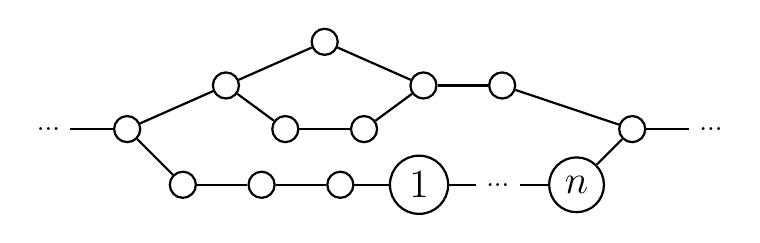
\begin{tikzpicture} [auto, node distance=1cm, every loop/.style={},
                    thick,solmu/.style={circle,draw,font=\sffamily\Large\bfseries}]

\node[solmu] (L) {};
\node[solmu] (TL)[above right= 0.3cm and 1cm of L] {};
\node[solmu] (T) [above right=0.3cm and 1cm of TL] {};
\node[solmu] (M1) [below right=0.3cm and 0.5cm of TL] {};
\node[solmu] (M2) [right of=M1] {};
\node[solmu] (TR1) [above right=0.3cm and 0.5cm of M2] {};
\node[solmu] (TR2) [right of=TR1] {};
\node[solmu] (B1) [below right of=L] {};
\node[solmu] (B2) [right of=B1] {};
\node[solmu] (B3) [right of=B2] {};
\node[solmu] (B4) [right of=B3] {$1$};
\node (B5) [right of=B4] {...};
\node[solmu] (B6) [right of=B5] {$n$};
\node (INVL) [left of=L] {...};
\node[solmu] (R) [above right of = B6] {};
\node (INVR) [right of=R] {...};

 \path[every node/.style={font=\sffamily\small}]
    (R) edge node[left] {} (INVR)
    (L) edge node[left] {} (INVL)
    (L) edge node[left] {} (TL)
    (TL) edge node[left] {} (T)
    (TL) edge node[left] {} (M1)
    (M1) edge node[left] {} (M2)
    (M2) edge node[left] {} (TR1)
    (T) edge node[left] {} (TR1)
    (TR1) edge node[left] {} (TR2)
    (TR2) edge node[left] {} (R)
    (L) edge node[left] {} (B1)
    (B1) edge node[left] {} (B2)
    (B2) edge node[left] {} (B3)
    (B3) edge node[left] {} (B4)
    (B4) edge node[left] {} (B5)
    (B5) edge node[left] {} (B6)
    (B6) edge node[left] {} (R);
\end{tikzpicture}
\end{center}
missä jokainen väri korvataan $n$ solmun ketjun sisältävällä aligraafilla, jossa $n$ vastaa värin numerointia. Aligraafin ylemmän komponentin orientaatio vastaa alkuperäisen kaaren suuntaa. Näin saadaan suuntaamaton, väritön graafi $G'$. Huomataan, että aligraafityypit eivät ole keskenään isomorfismisia, sillä jokainen sisältää eri määrän solmuja. Jokainen aligraafi sisältää täsmälleen yhden 5-syklin, joka on epäsymmetrisesti kiinnitetty aligraafiin. Muut aligraafin solmut määräytyvät 5-syklin mukaan. Graafi ei sisällä muita 5-syklejä, sillä jokainen muu sykli sisältää vähintään 6 solmua. Tästä seuraa se, että $\mathrm{Aut}(G) \simeq \mathrm{Aut}(G')$.
\end{proof}
\end{teor}

Roberto Frucht todisti Lauseen \ref{frucht} ensimmäisen kerran vuonna 1938 \cite{frucht1938herstellung}.

\bibliographystyle{plain}
\bibliography{aine}{}
\end{document}